 \documentclass[c]{beamer}
%\documentclass{beamer}
\listfiles

\mode<presentation>
{
  %\usetheme[deutsch,titlepage0]{KIT}
\usetheme[deutsch]{KIT}
% \usetheme{KIT}

%%  \usefonttheme{structurebold}

  \setbeamercovered{transparent}

  \setbeamertemplate{enumerate items}[circle]
  %\setbeamertemplate{enumerate items}[ball]

}
\usepackage{babel}
\date{}
%\DateText

\newlength{\Ku}
\setlength{\Ku}{1.43375pt}

\usepackage[utf8]{inputenc}
\usepackage[TS1,T1]{fontenc}
\usepackage{array}
\usepackage{multicol}
\usepackage{lipsum}
\usepackage[]{algorithm2e}
\usepackage{amsmath}
\usepackage{color}

\usenavigationsymbols
%\usenavigationsymbols[sfHhdb]
%\usenavigationsymbols[sfhHb]

\subtitle{Algorithmen I SS 14}
\author[]{Lena Winter}

\AuthorTitleSep{\relax}

\institute[ITI]{Institut für Theoretische Informatik}

\TitleImage[width=\titleimagewd]{images/title}

\newlength{\tmplen}

\newcommand{\verysmall}{\fontsize{6pt}{8.6pt}\selectfont}

\title[Algorithmen I SS 14]{Tutorium 11}

\usepackage{alltt}

\TitleImage[width=\titleimagewd]{images/title02}
\definecolor{OliveGreen}{RGB}{85,107,47}

\begin{document}

\begin{frame}
  \maketitle
\end{frame}


\begin{frame}{Union-Find Datenstruktur}
	Union-Find ist eine Partition einer Menge so, dass folgende Operationen effizient durchführbar sind:
	\begin{description}
		\item[union(x,y)] Vereinigt die Menge mit x mit der Menge mit y 
		\item[find(x)] Gibt den Repräsentanten der Menge mit x zurück
	\end{description}

	\textbf{Herausfinden ob x in der selben Menge wie y:} find(x) == find(y)

	\ \\
	Repräsentation der Mengen als Bäume: Repräsentanten sind Wurzel
\end{frame}

\begin{frame}{Beispiel Union-Find}
	Zu Beginn: Die Partition besteht aus n ein-elementigen Mengen
	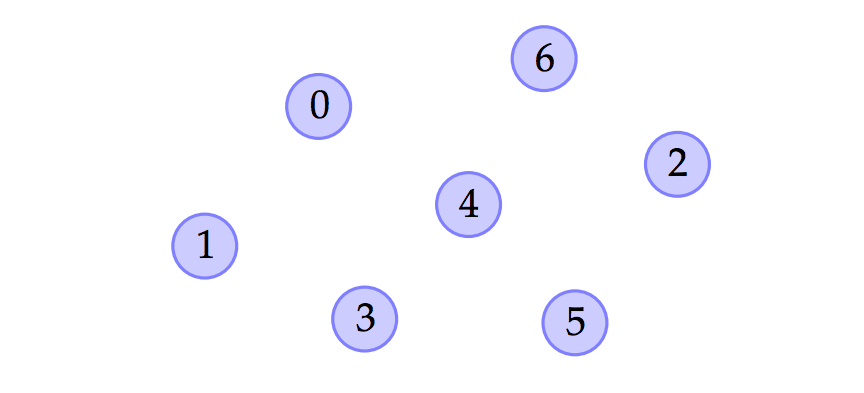
\includegraphics[width=\textwidth]{images/uf01}
	
\end{frame}

\begin{frame}{Beispiel Union-Find}
	union(4,6) \\
	\color{black}find(4) == find(6): \color{OliveGreen}{true} \\
	\color{black}find(1) == find(3): \color{red}{false} \\
	\color{black}find(5) == find(2): \color{red}{false} \\
	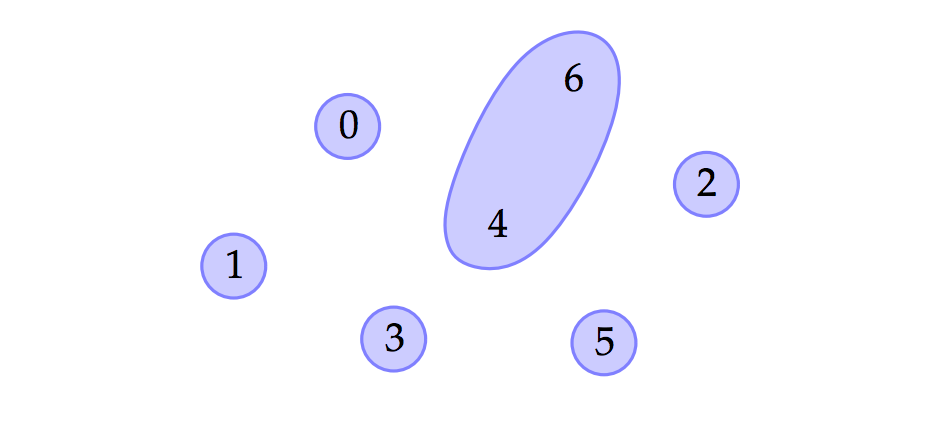
\includegraphics[width=\textwidth]{images/uf02}
	
\end{frame}

\begin{frame}{Beispiel Union-Find}
	union(1,3) \\
	\color{black}find(4) == find(6): \color{OliveGreen}{true} \\
	\color{black}find(1) == find(3): \color{OliveGreen}{true} \\
	\color{black}find(5) == find(2): \color{red}{false} \\
	
	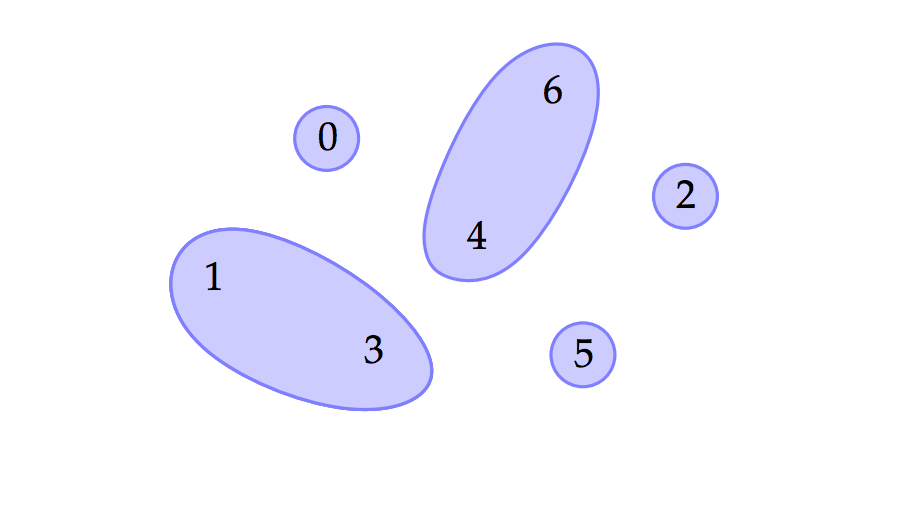
\includegraphics[width=\textwidth]{images/uf03}
	
\end{frame}

\begin{frame}{Optimierungen}
	\begin{description}
	\item[find()] Alle traversierte Knoten direkt an die Wurzel gehängt: \\
		$\rightarrow$ Reduziert Baumhöhe. 

	\item[union()] Der kleine Baum wird an den Größeren gehängt
	\end{description}	

\end{frame}

\begin{frame}{Laufzeit}
	\begin{itemize}
		\item Amortisierte Laufzeit pro Operation: $\mathcal{O}(\alpha(n))$
		\begin{itemize}
			\item $\alpha(n)$ ist die Inverse Ackermannfunktion
			\item sehr langsam wachsend:
		\end{itemize}
		\centerline{$\alpha( 2 ^ {2 ^{10 ^{19792}}}) < 5$}
	\end{itemize}
\end{frame}



\begin{frame}{Aufgabe: Bottleneck Shortest Path}
	Sei $G = (V, E)$ ein zusammenhängender ungerichteter gewichteter Graph und $s, t \in V$. Ein kreisfreier Pfad P zwischen s und t heiße ein Bottleneck Shortest Path (BSP) für s und t,
	wenn das größte in P auftretende Kantengewicht minimal ist für alle Pfade zwischen s und t
	\begin{enumerate}
		\item Zeigen Sie: Ist T ein MST in G, dann ist der in T eindeutige Pfad P zwischen zwei Knoten $s, t \in V$ ein BSP in G für s und t.
		\item Geben Sie einen Algorithmus an, der für gegebenen $G = (V, E)$, gegebene $s, t \in V$ und einen gegebenen MST T in G einen BSP P zwischen s und t ausgibt.
		Die Laufzeit soll dabei in $\mathcal{O}(|P|)$ liegen.
		Nehmen Sie an T liege in Form des Array \textit{parent} vor.
		\item Argumentieren Sie kurz warum ihr Algorithmus korrekt und die geforderte Laufzeit hat.
	\end{enumerate}

\end{frame}

\begin{frame}{Aufgabe Kürzeste Wege}
	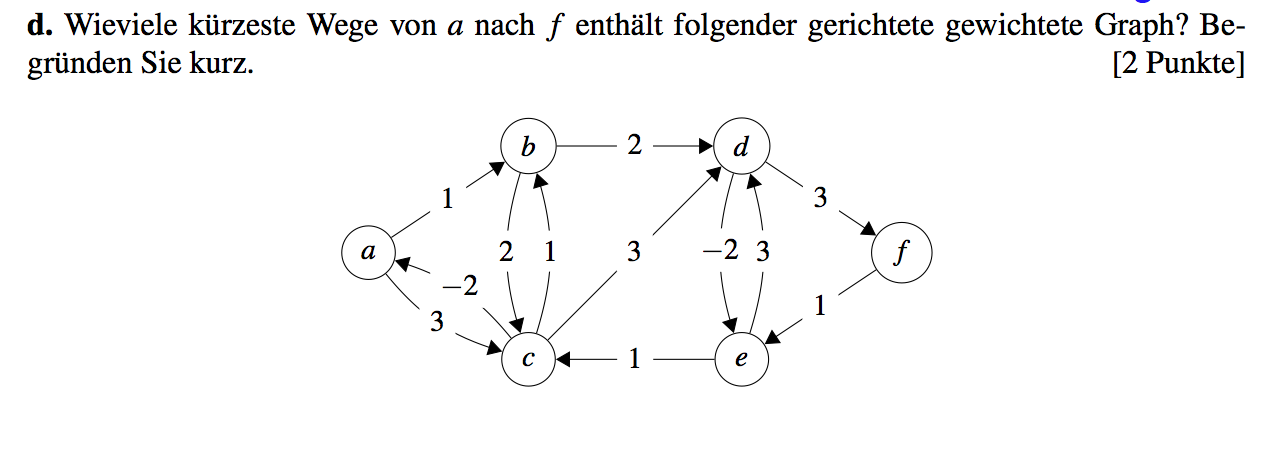
\includegraphics[width=\textwidth]{images/shortestPath01}
\end{frame}


\begin{frame}{Aufgabe Kürzeste Wege}
	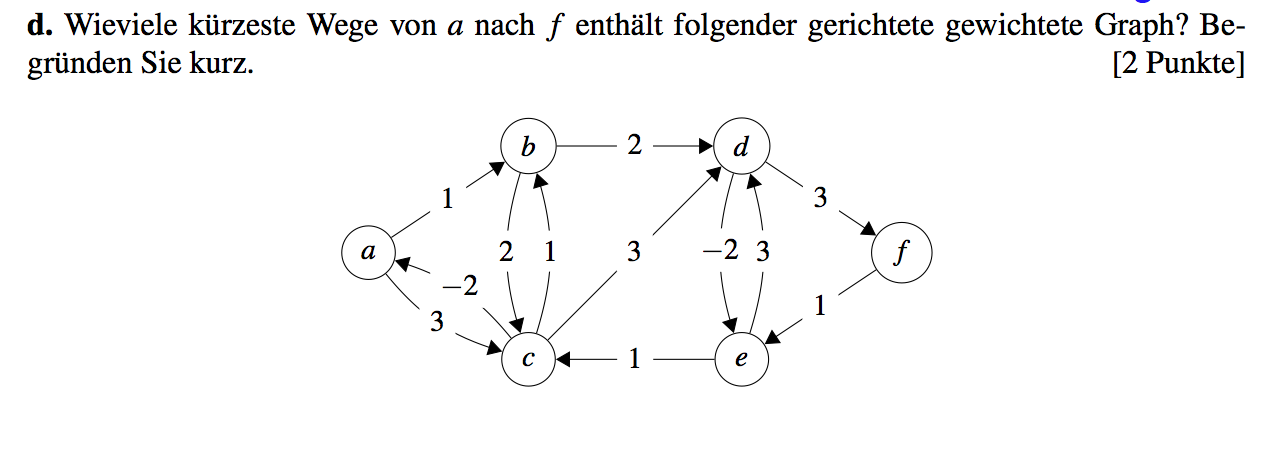
\includegraphics[width=\textwidth]{images/shortestPath01}
	\ \\
	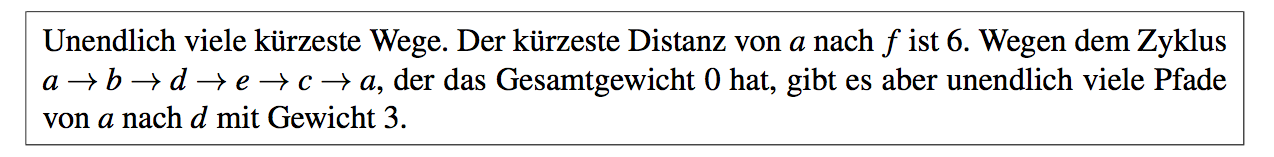
\includegraphics[width=\textwidth]{images/shortestPath02}
\end{frame}


\begin{frame}{Kreativaufgabe: Streaming MST}
	Gegeben sei ein zusammenhängender Graph mit $n$ Knoten und $m$ Kanten.
	Die Knoten sind lokal gespeichert, während die Kanten über eine Netzwerkverbindung gestreamt werden.
	Sie können nicht lokal gespeichert werden, da nur $\mathcal{O}(n)$ Speicherplatz vorhanden ist.

	\textbf{Aufgabe 1}: Gib einen Algorithmus an, der einen MST von G unter diesen Einschränkungen bestimmt.

	\textbf{Aufgabe 2}: Verbessere diesen Algorithmus so, dass er nur $\mathcal{O}(m \log{n})$ Rechenzeit benötigt.
\end{frame}

\end{document}
